\documentclass[12pt, oneside]{report}

\usepackage[left=3.5cm, top=2.5cm, bottom=2.5cm, right=2.5cm]{geometry}

\usepackage[utf8]{inputenc}
\usepackage[T1]{polski}
\usepackage[polish]{babel}
\usepackage{indentfirst}
\usepackage{graphicx}
\usepackage{mathtools}

\usepackage{natbib}


\begin{document}  
\thispagestyle{empty}
\begin{titlepage}
    \begin{center}

           \Large
	\textbf{Uniwersytet Jagielloński w Krakowie}\vspace{0.2cm}\\ Wydział Fizyki, Astronomii i Informatyki Stosowanej
               \vspace*{1cm}
               
         \vspace{3cm}
         \Large
          \textbf{Paweł Sławomir Mstowski}\\\vspace{0.5cm}
         \normalsize Nr albumu: 1148921\\
             \vspace{2cm}
        \Huge
        \textbf{Nauczanie sieci neuronowych za pomocą algorytmu genetycznego na przykładzie samouczącego się bota do gry zręcznościowej.}
      
        \vspace{1.5cm}
        \normalsize
        Praca magisterska\\
        na kierunku Informatyka Stosowana\\ \vspace{0.15cm}
        
        \vfill
        \vspace{2cm}
       \begin{minipage}{1\textwidth}
\begin{flushright}
Praca wykonana pod kierunkiem\\
prof. dr hab. Piotra Białasa\\
Zakład Technologii Gier
\end{flushright}
\end{minipage}
        
        \vspace{2cm}
        \begin{center}
      Kraków 2019
        \end{center}
    \end{center}
\end{titlepage}

\newpage 
 \thispagestyle{empty}
\vspace{2.5cm}
\begin{flushleft}
\large \textbf{Oświadczenie autora pracy}\vspace{0.6cm}\\
\end{flushleft}

\noindent Świadom odpowiedzialności prawnej oświadczam, że niniejsza praca dyplomowa została napisana przeze mnie samodzielnie i nie zawiera treści uzyskanych w sposób niezgodny z obowiązującymi przepisami.\\

\noindent Oświadczam również, że przedstawiona praca nie była wcześniej przedmiotem procedur związanych z uzyskaniem tytułu zawodowego w wyższej uczelni.
\vspace{2cm}
\begin{center}
\begin{tabular}{lr}
................................~~~~~~~~~~~~~~~~~~~~~~~~~~~~~~~~~~~~~~&
.......................................... \\
{~~~~Kraków, dnia} & {Podpis autora pracy~~~~}
\end{tabular}
\end{center}
\vspace{5cm}
\begin{flushleft}
\large \textbf{Oświadczenie kierującego pracą}
\end{flushleft}

\noindent Potwierdzam, że niniejsza praca została przygotowana pod moim kierunkiem i~kwalifikuje się do przedstawienia jej w postępowaniu o nadanie tytułu zawodowego.
\vspace{2cm}
\begin{center}
\begin{tabular}{lr}
................................~~~~~~~~~~~~~~~~~~~~~~~~~~~~~~~~~~~~~~&
............................................ \\
{~~~~Kraków, dnia} & {Podpis kierującego pracą~~}
\end{tabular}
\end{center}
\vfill
\tableofcontents

%%%%%%%%%%%%%%%%%%%%%%%%%%%%%%%%%%%%%%%%%%%%%%%%%%%%%%%%%%%%%%%%%%%%%%%%%%%%%%%%%%%%%


\chapter{Wprowadzenie}

%%%%%%%%%%%%%%%%%%%%%%%%%%%%%%%%%%%%%%%%%%%%%%%%%%%%%%%%%%%%%%%%%%%%%%%%%%%%%%%%%%%%%

\chapter{Sieci neuronowe}
\section{Czym są sieci neuronowe?}

Sieci neuronowe są to systemy przetwarzania informacji wzorowane na procesach i strukturach obserwowanych w ludzkim mózgu. Pierwszą sztuczną siecią neuronową był perceprton progowy, który został wymyślony w roku 1943 przez Warrena Sturgisa McCullocha i Waltera Pittsa. Wymyślona wtedy koncepcja jest nadal bardzo aktualna i wykorzystywana do dziś. Teraźniejszy poziom zaawansowania komputerów i ich moc obliczeniowa wywołały swego rodzaju renesans badań nad sieciami neuronowymi.

Tak samo jak nasz mózg składa się z setek miliardów komórek neuronowych tak sztuczne sieci neuronowe są tworzone przez setki lub tysiące sztucznych neuronów, które są najmniejszymi elementami przetwarzającymi informację. Są one prymitywną interpretacją sposobu działania prawdziwych, biologicznych neuronów i składają się z wielu wejść oraz jednego wyjścia. Budowa takiego pojedynczego elementu sieci przedstawiona jest poniżej (Rysunek \ref{fig: 2.1}).

\begin{figure}[h]
	\centering
	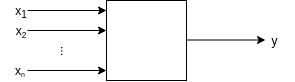
\includegraphics[width=7cm]{fig211.png}
	\caption{Schemat budowy sztucznego neuronu}
	\label{fig: 2.1}
\end{figure}

Każde wejście sztucznego neuronu posiada też swoją wagę, która jest potem używana do obliczenia jego wyjścia. W takim wypadku funkcję każdego pojedynczego elementu sieci możemy zapisać jako (Równanie \ref{eq: 2.1})

\begin{equation}\label{eq: 2.1}
y = \sum^{n}_{i=1} x_{i}w_{i}
\end{equation}
\pagebreak

Dodatkowo każdy neuron posiada swoją wartość przesunięcia (ang. \textit{bias}) sygnału. Funkcja wyjścia zaprezentowana powyżej z uwzględnieniem tej wartości będzie wyglądać (Równanie \ref{eq: 2.2}):

\begin{equation}\label{eq: 2.2}
  y = \sum^{n}_{i=1} x_{i}w_{i} + b
\end{equation}

Topologia połączeń oraz ich parametry stanowią program działania sieci \cite{tadeusiewicz1993sieci}. Sygnały wejściowe są przepuszczane przez chmurę połączonych ze sobą neuronów, które następnie przeliczają te sygnały i przekazują swoje rozwiązania dalej w głąb sieci. Tak przetworzone dane dają w wyniku pewną ilość sygnałów wyjściowych z sieci które razem są rozwiązaniem problemu, do którego została wyuczona.

Możemy wyodrębnić kilka podstawowych rodzajów sieci neuronowych na podstawie ich topologii takie jak sieci jedno warstwowe, wielowarstwowe, jednokierunkowe czy rekurencyjne. Każda z tych wariacji jest skuteczna w rozwiązywaniu innych problemów. Dla przykładu sieci jednowarstwowe, które w praktyce składają się z dwóch warstw (warstwa wejściowa nie przetwarza a jedynie przekazuje dane wejściowe do sieci), nadają się do klasyfikowania informacji, które jesteśmy w stanie rozdzielić liniowo. Sieci wielowarstwowe różnią się od jednowarstwowych jedynie dodatkowymi warstwami ukrytymi. W klasycznych sieciach neuronowych połączenia pomiędzy neuronami istnieją jedynie między warstwami. Obraz poniżej prezentuje przykładową wielowarstwową sztuczną sieć neuronową (Rysunek \ref{fig: 2.2})

\begin{figure}[h]
	\centering
	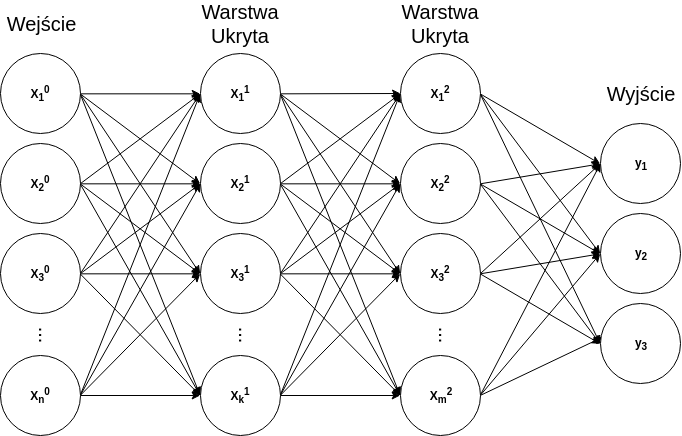
\includegraphics[width=12cm]{fig212.png}
	\caption{Schemat wielowarstwowej sieci neuronowej}
	\label{fig: 2.2}
\end{figure}

Aby jednoznacznie określić konkretną sztuczną sieć neuronową możemy się posłużyć uproszczonym modelem opisanym przez trzy podstawowe cechy takiej sieci. Tymi cechami są architektura, proces uczenia i funkcja aktywacji. Architektura opisuje dokładnie topologię sieci, w tym jej rodzaj oraz liczby warstw i neuronów w każdej warstwie. Uczenie jest opisem procesu zastosowanego do rozwinięcia parametrów sieci. Określa ono poszczególne techniki użyte do tego celu jak na przykład uczenie przez wzmacnianie czy uczenie ze zbioru reguł. Definiuje też zakresy i wartości wag połączeń między neuronami. Ostatnia cecha czyli funkcja aktywacji opisuje sposób wewnętrznego działania neuronu, czyli kiedy będzie on aktywny oraz jakie dane przekaże dalej w głąb sieci.

Istnieje wiele powszechnie używanych funkcji aktywacji neuronów. Najprostszym jej przykładem jest funkcja tożsamości, która przekazuje bezpośrednio na wyjście wartość aktywacji neuronu i jest wyrażana wzorem (Równanie \ref{eq: 2.3})

\begin{equation}\label{eq: 2.3}
  f(a) = a
\end{equation}

Innym przykładem jest funkcja nazywana \textbf{ReLU}(\textit{Rectified Linear Unit}) i najbardziej ze wszystkich odzwierciedla sposób aktywacji neuronu biologicznego (Równanie \ref{eq: 2.4}).

\begin{equation}\label{eq: 2.4}
    f(a) =
    \begin{cases*}
      a & if a $\geq$ 0 \\
      0 & if a < 0
    \end{cases*}
\end{equation}

Powyższa funkcja jest połączeniem funkcji tożsamości oraz funkcji progowej, która na wyjściu zwraca tylko informację czy została aktywowana i opisuje ją wzór (Równanie \ref{eq: 2.5})

\begin{equation}\label{eq: 2.5}
  f(a) =
  \begin{cases*}
    1 & if a $\geq$ 0 \\
    0 & if a < 0
  \end{cases*}
\end{equation}

Istnieją również bardziej zaawansowane funkcje aktywacji. Jedną z najczęściej używanych jest funkcja logistyczna (Równanie \ref{eq: 2.6}), która zwraca wartość mięczy 0 a 1 i jej wynik jest określany jako prawdopodobieństwo aktywacji neuronu.

\begin{equation}\label{eq: 2.6}
  f(a) = \frac{1}{1 + exp(-a)}
\end{equation}

\section{Zastosowania sieci neuronowych}

Bazując na wcześniej podanych informacjach można powiedzieć, że sztuczne sieci neuronowe pomimo swojej genezy nie są idealnym odzwierciedleniem sposobu działania swojego pierwowzoru, czyli ludzkiego mózgu. Przez swoje ograniczenia ich zdolności do rozwiązywania problemów są ograniczane. Każda sieć neuronowa jest projektowana i uczona do rozwiązywania konkretnego problemu i nie radzi sobie z danymi związanymi z innymi zagadnieniami niż jej specjalizacja. Z podstaw działania sztucznego neuronu można wywnioskować, że ma on zdolność do rozpoznawania wzorców na podstawie porównania otrzymanych sygnałów do swojego wektora wag. Z tego wynika, że sztuczne neurony połączone w skomplikowaną sieć są idealne do takich zadań na dużo większą skalę. Taki sposób działania pozwala na wykorzystanie tych mechanizmów w wielu branżach.

Aktualnie sieci neuronowe są używane do przetwarzania danych w bardzo dużym spektrum dziedzin. Ich zastosowania można znaleźć przedmiotach codziennego użytku takich jak smartfony, na przykład do rozpoznawania mowy i implementacji interfejsów głosowych, jak też w bardzo profesjonalnych sprzętach i systemach. Na podstawie wcześniej dostarczonych danych jesteśmy w stanie nauczyć sieci neuronowe przewidywać pewne zdarzenia na podstawie aktualnych danych. Wiele firm w dzisiejszych czasach tworzy systemy, które na podstawie parametrów technicznych urządzeń w zakładach są wstanie podać bardzo dokładne prawdopodobieństwo awarii danego sprzętu. Sztuczne sieci neuronowe zostały wykorzystane przez różnych badaczy do modelowania i prognozowania w dziedzinie systemów inżynierii energetycznej \cite{kalogirou2000applications}. Współczesna medycyna generuje zawrotne ilości danych korzystając z zaawansowanych czujników monitorujących. Potencjalne zastosowania takich danych obejmują dokładne klasyfikowanie diagnoz, przewidywanie przyszłych chorób i śmiertelności \cite{lipton2015learning}.

Zastosowanie sieci neuronowych w dzisiejszych czasach jest bardzo dobrze widoczne w dziedzinie rozpoznawania obrazów. Wydajność i dokładność algorytmów tworzonych do tych celów może być w łatwy sposób mierzona poprzez porównanie wyniów ich działania na popularnej bazie ImageNet \cite{image-net} zawierającej szesnaście milionów zdjęć. W czasach małej popularności sieci neuronowych sprawność algorytmów rozpoznawania obrazów rozwijała się bardzo powoli. Jednakże w okresie wzmożonego wprowadzania rozwiązań z tematyki sieci neuronowych do tejże dziedziny możemy zaobserwować znaczny spadek stopy błędu z 40\% w roku 2010 do zaledwie 7\% w roku 2014. Ze względu na sukces głębokich sieci neuronowych wszyscy uczestnicy współzawodnictwa ImageNet w 2013 roku zastosowali jakąś formę głębokiej sieci neuronowej \cite{roelants2017deeplearning}.

Często wyuczone sieci odzwierciedlają swoim działaniem algorytmy, które już zostały wymyślone. Jednakże sposób w jaki to robią może dostarczyć nowych spostrzeżeń dotyczących rozwiązywanego problemu i lepszych implementacji algorytmów \cite{murray1995applications}.


\section{Metody nauczania sieci neuronowych}

Pod pojęciem nauczania sieci neuronowej, zwanego też uczeniem maszynowym, kryją się różne procesy prowadzące do takiej modyfikacji wszystkich wag w sieci aby jak najlepiej rozwiązywała dany problem. Techniki uczenia maszynowego można zgrubnie podzielić na dwie duże klasy: uczenie nadzorowane i nienadzorowane, choć dość często dodawana jest też trzecia klasa - tzw. uczenie przez wzmacnianie \cite{roelants2017deeplearning}. Każda z tych klas wymaga dostarczenia innych danych do poprawnego działania. W niektórych przypadkach musimy dysponować dużą ilością informacji wstępnie sklasyfikowanych, żeby sieć na ich przykładzie mogła się uczyć a w innych potrzebujemy po prostu surowych danych, które taka sieć sklasyfikuje samodzielnie.

Uczenie nadzorowane jest pierwsza wymienioną przeze mnie klasą algorytmów nauczania maszynowego. Zaliczają się do niej algorytmy korzystające z zestawów danych treningowych, które są wstępnie opracowywane i oznaczane oczekiwanymi etykietami (etykietowane) ręcznie przez osoby nadzorujące uczenie sieci. Samo uczenie odbywa się poprzez zmiany w zestawie wag sieci, które dążą zo zminimalizowania wartości funkcji błędu określanej przez różnicę między wyjściem sieci a właśnie oczekiwanymi etykietami. W konsekwencji działania takiego algorytmu otrzymujemy sieć neuronową, której wagi wyznaczają \textit{k-1} hiperpłaszczyzn w \textit{n-wymiarowej} przestrzeni, gdzie \textit{k} jest liczbą oczekiwanych klas a \textit{n} ilością neuronów wejściowych sieci.

Kolejną klasą algorytmów jest uczenie nienadzorowane, które stając po przeciwnej stronie do poprzednio zaprezentowanego uczenia nadzorowanego nie korzysta z wcześniej etykietowanych danych. Najlepszym przykładem działania tych algorytmów jest grupowanie otrzymanych danych poprzez wyszukanie odpowiedniej ilości klas danych tak aby poszczególne elementy tych grup cechowały się jak największym podobieństwie do siebie i jak najmniejszym podobieństwem do elementów innych grup.

Ostatnią zaprezentowaną klasą algorytmów było uczenie przez wzmacnianie. Działa ono podobnie do nienadzorowanego ale wykorzystuje też mechanikę sprzężenia zwrotnego z uczenia nadzorowanego.

%%%%%%%%%%%%%%%%%%%%%%%%%%%%%%%%%%%%%%%%%%%%%%%%%%%%%%%%%%%%%%%%%%%%%%%%%%%%%%%%%%%%%

\chapter{Algorytm genetyczny}
\section{Powstanie algorytmu genetycznego}
\section{Problem kodowania rozwiązania}
\section{Zastosowania}

%%%%%%%%%%%%%%%%%%%%%%%%%%%%%%%%%%%%%%%%%%%%%%%%%%%%%%%%%%%%%%%%%%%%%%%%%%%%%%%%%%%%%

\chapter{Wykorzystanie algorytmu genetycznego w nauczaniu sieci neuronowych}

%%%%%%%%%%%%%%%%%%%%%%%%%%%%%%%%%%%%%%%%%%%%%%%%%%%%%%%%%%%%%%%%%%%%%%%%%%%%%%%%%%%%%

\chapter{Samouczący się bot do gry zręcznościowej}
\section{Stos technologiczny}
\section{Struktura projektu}
\section{Zastosowane techniki sztucznej inteligencji}\textsl{}
\section{Opis działania}

\chapter{Wnioski}

\pagebreak
%%%%%%%%%%%%%%%%%%%%%%%%%%%%%%%%%%%%%%%%%%%%%%%%%%%%%%%%%%%%%%%%%%%%%%%%%%%%%%%%%%%%%
\bibliographystyle{plain}
\bibliography{bibliography}
\end{document}